\documentclass[10pt]{article}
\usepackage[margin=0.72in]{geometry}
\usepackage[T1]{fontenc}
\usepackage{lmodern}
\usepackage{amsmath,amssymb,amsthm,mathtools}
\usepackage{microtype}
\usepackage{titlesec}
\usepackage{xcolor,enumitem,booktabs,tabularx,array}
\usepackage{pgfplots}
\pgfplotsset{compat=1.18}
\usepackage[hidelinks]{hyperref}
\titlespacing*{\section}{0pt}{1.2ex plus 0.4ex minus 0.2ex}{0.6ex plus 0.2ex}
\titlespacing*{\subsection}{0pt}{0.9ex plus 0.3ex minus 0.2ex}{0.4ex plus 0.2ex}
\setlength{\abovedisplayskip}{6pt plus 2pt minus 2pt}
\setlength{\belowdisplayskip}{6pt plus 2pt minus 2pt}
\setlength{\parskip}{3pt}
\setlength{\parindent}{0pt}
\setlist{nosep,leftmargin=1.5em}
\newcommand{\E}{\mathbb E}
\newcommand{\KL}{\operatorname{KL}}
\newcommand{\N}{\mathcal N}
\newcommand{\II}{\mathrm I}
\newcommand{\dd}{\mathrm d}
\newcommand{\Score}[1]{E_{\mathrm{score},#1}}
\newcommand{\sg}{\operatorname{sg}}
\newcommand{\D}{\mathcal D}
\newcommand{\one}{\boldsymbol{1}}
\hypersetup{pdftitle={Hierarchical Iterative CSEM Cotraining},pdfsubject={Direct-latent cascade, conditional CSEM, cutoff closure and 500-epoch Fashion-MNIST results}}
\begin{document}
\begin{center}
{\Large\bfseries Hierarchical Iterative CSEM Cotraining}\\[3pt]
{\large Conditional Diffusion Priors, Direct-Latent Cascades, and Cutoff Closure}\\[5pt]
{\small Updated 13 October 2026 --- Architecture and experimental research note}
\end{center}
\vspace{-0.8em}
\begin{abstract}
A hierarchical VAE can have conditionally Gaussian encoder blocks and expressive non-Gaussian aggregate conditional priors learned by sequential diffusion.  The \emph{default} architecture is now a two-block \emph{direct-latent} cascade: the child posterior, conditional CSEM score head, terminal regularizer and decoder all use the same stochastic variable $Z_2$, without a decoder-only root-dependent affine transformation. The child posterior sees bottom-up image features and top-down clean-root features, whereas the decoder reconstructs from \emph{both OU-corrupted codes} and recomputes every root-dependent feature from the corrupted root. Clean ancestors are reserved for conditional score supervision and sampling. We retain the exact conditional CSEM information identity, distinguish it from the implemented unit-epsilon/log-time weighting, and explain the positive-cutoff $B_{t_{\min}}$ bound. A completed, single-seed, 500-epoch Fashion-MNIST run gives \textbf{Gaussian-start generated FID 4.8983} with two sequential RK4-20 solves, classifier-free guidance 3, and 10,000-image legacy Inception evaluation. This improves on our previously documented terminal-KL Gaussian-start result (5.13 with Heun-50) under a different solver protocol. Root/child gradients, posterior variance, conditional generation and child-ablation probes demonstrate a functioning hierarchy, but do not directly identify the blockwise mutual information or establish a controlled causal advantage over all flat designs.
\end{abstract}

\section{Conditional hierarchy and exact score targets}
For $M$ stochastic blocks, write $Z_{<i}=(Z_1,\ldots,Z_{i-1})$ and
\begin{equation}
q_\phi(z_{1:M}\mid x)=\prod_{i=1}^M q_{\phi_i}(z_i\mid x,z_{<i}),\qquad
q_{\phi_i}(z_i\mid x,a)=\N\bigl(\mu_i(x,a),\Sigma_i(x,a)\bigr).
\label{eq:encoder}
\end{equation}
Covariances can be diagonal even when the networks producing their parameters are deep and multiscale. Image features may enter posterior inference, but the generative decoder receives only latent variables and deterministic features derived from them. Under the joint law $p_{\rm data}(x)q_\phi(z_{1:M}\mid x)$, the aggregate factor is
\begin{equation}
q_{\phi,i}(z_i\mid a)=\int q_\phi(x\mid a)q_{\phi_i}(z_i\mid x,a)\,\dd x.
\label{eq:aggregate}
\end{equation}
It is generally a Gaussian mixture, not a Gaussian prior. Learn each factor using a conditional diffusion head, yielding $p_\theta(z_{1:M})=\prod_i p_{\theta_i}(z_i\mid z_{<i})$.

Use the OU convention $\alpha_t=e^{-t}$, $\gamma_t=1-e^{-2t}$, $\sigma_t=\sqrt{\gamma_t}$ and $Y_{i,t}=\alpha_tZ_i+\sigma_t\xi_i$, $\xi_i\sim\N(0,I)$. Hold the \emph{clean sampled} ancestors $a=Z_{<i,0}$ fixed while diffusing block $i$. Then
\begin{align}
q_{\phi,i,t}(y\mid x,a)&=\N(\alpha_t\mu_i,S_{i,t}), & S_{i,t}&=\alpha_t^2\Sigma_i+\gamma_tI,\\
C_{i,t}(y;x,a)&=-S_{i,t}^{-1}(y-\alpha_t\mu_i), & \epsilon^*_{i,t}&=-\sigma_t C_{i,t}.
\label{eq:targets}
\end{align}
The head sees $(Y_{i,t},t,a)$, plus an optional class label, but never $X$. For diagonal variance $v_i$, its unit-epsilon target is elementwise
\begin{equation}
\epsilon^*_{i,t}=\frac{\sigma_t(Y_{i,t}-\alpha_t\mu_i)}{\alpha_t^2v_i+\sigma_t^2}.
\label{eq:eps}
\end{equation}
The population minimizer is the conditional aggregate score $\nabla_y\log q_{\phi,i,t}(y\mid a)$. Equations suppress label conditioning: when a head sees a class or dropout label, condition its aggregate score and the information identities on that available label as well. ``Clean'' denotes absence of extra OU corruption, not a posterior mean or a deterministic root.

\section{Canonical information identity}
Define the unnormalized score-space integral $L_i^{0:T}=\int_0^T\E\|s_{\theta_i}-C_{i,t}\|^2\dd t$, the aggregate-score approximation error $\Score{i}^{0:T}=\int_0^T\E\|s_{\theta_i}-\bar s_{i,t}\|^2\dd t$, and
\begin{equation}
K_{i,T}=\E_{X,A}\KL\!\left(\N(\alpha_T\mu_i,S_{i,T})\,\middle\|\,\N(0,I)\right).
\end{equation}
Here $A=Z_{<i,0}$ and $\bar s_{i,t}=\nabla\log q_{\phi,i,t}(\cdot\mid A)$. Conditional OU information dissipation, regression orthogonality and the KL chain rule give
\begin{equation}
\boxed{L_i^{0:T}+K_{i,T}=\II(X;Z_i\mid A)+\Score{i}^{0:T}
+\E_A\KL\bigl(q_{\phi,i,T}(\cdot\mid A)\|\N(0,I)\bigr).}
\label{eq:identity}
\end{equation}
With a shared canonical coefficient, the information terms sum to $\II(X;Z_{1:M})$. This population identity assumes the stated OU clock, canonical time weighting, finite integrals and the usual differentiation regularity. A minibatch CSEM value includes intrinsic conditional information dissipation as well as head error; it is not an isolated measure of score learnability.

\medskip
\section{Default architecture: two-stage direct-latent cascade}\label{sec:directarch}
We use one notation, $Z_1,Z_2$, for \emph{both stochastic codes produced by the diffusion priors and consumed by the decoder}. The working Fashion-MNIST model has 256 coordinates:
\begin{center}
\begin{tabular}{@{}llll@{}}
\toprule
Block & Tensor shape & Coordinates & Learned generative factor\\
\midrule
Coarse root $Z_1$ & $4\times4\times4$ & 64 (25\%) & $p_{\theta_1}(z_1\mid c)$\\
Fine child $Z_2$ & $3\times8\times8$ & 192 (75\%) & $p_{\theta_2}(z_2\mid z_1,c)$\\
\bottomrule
\end{tabular}
\end{center}
The image encoder follows the recovered Fashion-MNIST feature backbone ($32\to16\to8$ spatial stages). A further $8\to4$ strided residual/attention stage predicts root Gaussian parameters. From a clean reparameterized root sample, top-down residual/attention blocks and a $4\to8$ upsampler construct $H(z_1)$. A child Gaussian posterior combines the $8\times8$ bottom-up image feature $F_8(x)$ with $H(z_1)$:
\begin{align}
q_{\phi_1}(z_1\mid x)&=\N\!\left(\mu_1(x),\operatorname{diag}v_1(x)\right),\\
q_{\phi_2}(z_2\mid x,z_1)&=\N\!\left(\mu_2(F_8(x),H(z_1)),\operatorname{diag}v_2(F_8(x),H(z_1))\right).
\label{eq:directpost}
\end{align}
Both $Z_1$ and $Z_2$ are reparameterized posterior samples and retain differentiable ancestor dependencies. There is \emph{no} separate innovation $U_2$, $b_2(z_1)$, or learned decoder-only scale $d_2(z_1)$. The \textbf{same $Z_2$} is diffused to $Y_{2,t}$ for CSEM, regularized by terminal KL and $B_{t_{\min}}$, generated by the child reverse solve, and supplied directly to the image decoder:
\begin{equation}
\widehat X=D_\psi(Z_1,Z_2;\tau_{\rm decode}),\qquad
D_\psi(z_1,z_2;\tau)=D_{\psi,8\to16\to32}\!\left(\mathrm{Fuse}\bigl(H(z_1),\mathrm{Conv}(z_2)\bigr);\tau\right).
\label{eq:directdecode}
\end{equation}
The root still provides \emph{deterministic multiscale skip features}; image-encoder features do not skip into the decoder. The child score head receives $(Y_{2,t},t,Z_{1,0},c)$, including full spatial root information: projected $4\times4$ root tokens, $8\times8$ spatial injection, and cross-attention in each DiT transformer block. The head never sees $x$ or the image-conditioned posterior moments as inputs. The latter, $\mu_2$ and $v_2$, define its analytic teacher target \eqref{eq:eps}; the learned score is that of the \emph{aggregate conditional} $q_{\phi,2,t}(y\mid z_1,c)$.

The default FMNIST configuration uses a 6,368,847-parameter VAE, a 5,488,836-parameter root DiT, and a 6,678,283-parameter conditional child DiT (counts from the completed run). The two heads are trained jointly with the VAE but sampled sequentially, root first and child conditioned on the completed root. The residual-affine predecessor is retained below only as historical evidence, not as the recommended design.

\textbf{Why direct coordinates?} In the predecessor, diffusion acted on $U_2$ while the decoder consumed $b_2(Z_1)+d_2(Z_1)\odot U_2$. At fixed root the map can be invertible and preserve conditional mutual information, but it need not preserve the OU geometry or finite-capacity CSEM regularity. Using $Z_2$ directly removes this unregularized decoder-coordinate transformation while keeping ordinary deterministic root-to-decoder features. This design principle is motivated by consistency; the present run does not isolate it causally from other historical changes.

\section{Clean conditional inference versus noisy reconstruction}
Clean ancestors are required by the \emph{conditional Gaussian CSEM target} and the conditional child sampler, not by the auxiliary image reconstruction loss. The actual data flow is:
\begin{center}
\begin{tabularx}{\linewidth}{@{}lXX@{}}
\toprule
Consumer & Root supplied & Child supplied\\
\midrule
Child posterior $q_{\phi_2}$ & Clean posterior sample $Z_{1,0}$ & Image features and top-down root features determine $q(Z_2\mid X,Z_{1,0})$\\
Root CSEM head & Corrupted root $Y_{1,t}$ & None\\
Child CSEM head and target & Clean $Z_{1,0}$ as conditioning & Corrupted \emph{direct} child $Y_{2,t}$, with analytic $\mu_2,v_2$ target\\
Training image decoder & Corrupted root $Y_{1,\tau}$ & Corrupted child $Y_{2,\tau}$\\
Generation image decoder & Completed root reverse sample & Completed conditional child reverse sample\\
\bottomrule
\end{tabularx}
\end{center}
Write $Y_{i,\tau}=\alpha_\tau Z_{i,0}+\sigma_\tau\xi_i$. In the actual training step, the sampled \emph{reconstruction corruption time} $\tau$ equals the sampled score time $t$, and the image loss uses
\begin{equation}
\widehat X_\tau=D_\psi(Y_{1,\tau},Y_{2,\tau};\tau),\qquad \tau=t\ \text{in the implemented minibatch}.
\label{eq:recontime}
\end{equation}
The semicolon separates the decoder time embedding from the two noisy inputs. One could in principle sample a distinct $\widetilde t$ for the reconstruction objective, but the reported run does not: $D(Y_{1,\widetilde t},Y_{2,\widetilde t};\widetilde t)$ would be a separately sampled corruption level, \emph{not} a clean code paired with an arbitrary time label. Decoder residual features $H$ are \textbf{always recomputed from $Y_{1,\tau}$}. Passing a cached $H(Z_{1,0})$ would create a clean-root shortcut and undermine child usage. For sampling, $D_\psi(\widehat Z_1,\widehat Z_2;\tau_{\rm decode})$ receives the completed reverse trajectories with the specified small decoding-time embedding.

By contrast, the child score is conditioned on $Z_{1,0}$, not $Y_{1,t}$. Changing its context to a noisy root while keeping the target conditional on the clean root would generally invalidate Gaussian supervision: conditioning on a noisy ancestor entails a mixture over latent clean roots. This clean-score/noisy-reconstruction distinction is a feature, not an inconsistency. The previous \emph{clean-root reconstruction} ablation $D_\psi(Z_{1,0},Y_{2,\tau};\tau)$ did collapse child use; the historical numbers are preserved in Section~\ref{sec:historical}.

\newpage
\section{Positive time cutoff and the \texorpdfstring{$B_{t_{\min}}$}{B at t min} term}
Let $t_0=t_{\min}>0$. The canonical truncated identity is
\begin{equation}
L_i^{t_0:T}+K_{i,T}=\II(X;Y_{i,t_0}\mid A)+\Score{i}^{t_0:T}
+\E_A\KL\bigl(q_{\phi,i,T}(\cdot\mid A)\|\N(0,I)\bigr).
\label{eq:truncated}
\end{equation}
Thus it charges the information surviving at $t_0$, not all the information in the clean block. When $v_i\ll\sigma_{t_0}^2/\alpha_{t_0}^2$, diffusion hides further posterior sharpening from the truncated integral. Define
\begin{equation}
\delta_0=\frac{\sigma_{t_0}^2}{\alpha_{t_0}^2}=e^{2t_0}-1,\qquad
B_i=\frac12\E_{X,A}\log\det\bigl(I+\delta_0\Sigma_i^{-1}\bigr).
\label{eq:band}
\end{equation}
For the Gaussian components in \eqref{eq:encoder},
\begin{equation}
0\le\II(X;Z_i\mid A)-\II(X;Y_{i,t_0}\mid A)\le B_i.
\label{eq:bandbound}
\end{equation}
There is no additive constant in this bound. It is an \emph{upper bound}, not an exact formula for the omitted information.

\subsection{Why the bound holds}
Given $A$, the Markov chain is $X\to Z_i\to Y_{i,t_0}$. Information lost to corruption equals $\II(X;Z_i\mid Y_{i,t_0},A)$. Dividing $Y$ by $\alpha_{t_0}$ gives the observation $W=Z_i+\sqrt{\delta_0}\xi$. Conditional on $(X,A,W)$, Gaussian conditioning yields
\begin{equation}
\Sigma_{\rm post}=(\Sigma_i^{-1}+\delta_0^{-1}I)^{-1}.
\end{equation}
Since $Z_i-W=-\sqrt{\delta_0}\xi$, conditional entropy obeys
\begin{align}
h(Z_i\mid W,A)&\le\frac{n_i}{2}\log(2\pi e\delta_0),\\
h(Z_i\mid X,W,A)&=\frac12\E_{X,A}\log\det(2\pi e\Sigma_{\rm post}).
\end{align}
Subtracting proves \eqref{eq:bandbound}. Consequently, with shared canonical coefficients, $L_i^{t_0:T}+K_{i,T}+B_i$ upper-bounds the right-hand side of \eqref{eq:identity}, with score error integrated only over $[t_0,T]$.

\subsection{Diagonal implementation and variance pressure}
For $n_i$ coordinates with log variances $\ell_{i,k}$, the script uses the per-coordinate mean
\begin{equation}
\overline B_i=\frac{1}{2n_i}\sum_{k=1}^{n_i}\operatorname{softplus}(\log\delta_0-\ell_{i,k}),\qquad
\frac{\partial B_{i,k}}{\partial\ell_{i,k}}=-\frac12\frac{\delta_0}{v_{i,k}+\delta_0}.
\label{eq:bandslope}
\end{equation}
Here $B_{i,k}=\tfrac12\log(1+\delta_0/v_{i,k})$. Its slope approaches $-1/2$ far below the cutoff scale and vanishes far above it: minimizing it discourages extreme sharpening. It is a \emph{soft penalty}, not a hard variance clamp. At $t_0=2\times10^{-5}$, the posterior standard-deviation threshold is approximately $\sqrt{\delta_0}=0.00632$, or log variance $-10.13$.

Compute the child penalty from $v_2(X,Z_{1,0})$ in the \emph{direct $Z_2$ coordinates}, with gradients through both variance and clean ancestors. The bound may be conservative; it does not guarantee useful allocation of information between blocks. In particular, a child posterior near an uninformative unit Gaussian can have a tiny band penalty and still be unused.

\subsection{Relation to learned-prior KL training}
For a learned-prior latent model, $\E_X\KL(q_\phi(z\mid X)\|p_\theta(z))=\II(X;Z)+\KL(q_{\phi,\rm agg}\|p_\theta)$. Both this and canonical CSEM impose information pressure, with different modeling remainders. The cutoff closure compensates conservatively for a truncated CSEM information budget; it should not be identified with an exact encoder entropy term, a learned-prior likelihood, or a score-head fitting loss. Terminal aggregate mismatch remains the distinct Gaussian-start anchoring mechanism.

\newpage
\section{Implemented objective and cotraining gradients}
\subsection{Coordinate averaging and time weighting}
For the two blocks, $n_1=64$, $n_2=192$, $n=n_1+n_2=256$ and $w_i=n_i/n$, giving $w_1=1/4$, $w_2=3/4$. Let
\begin{equation}
\ell_i=\E_{t,X,A,\xi}\frac{\|\widehat\epsilon_{\theta_i}(Y_{i,t},t,A)-\epsilon^*_{i,t}\|^2}{n_i},\quad
\overline K_i=K_{i,T}/n_i,\quad
\ell_C=\sum_iw_i\ell_i,\quad \ell_K=\sum_iw_i\overline K_i,\quad \ell_B=\sum_iw_i\overline B_i.
\end{equation}
This averages all coordinates rather than treating differently sized blocks equally. Applied to canonical score-space integrals and full KL/band terms, this normalization gives the summed information budget divided by $n$.

\textbf{The practical CSEM time weight is not canonical.} The script samples uniformly from a logarithmic grid of $N_t=1000$ times and uses unit-epsilon MSE. Because $\widehat\epsilon=-\sigma_t s_\theta$, its score-space time weight is approximately
\begin{equation}
\lambda(t_j)=\frac{\sigma_{t_j}^2}{N_t\,\Delta t_j},\qquad
\lambda(t)\simeq\frac{\sigma_t^2}{t\log(T/t_0)}.
\label{eq:lambda}
\end{equation}
Near zero, $\lambda(t)\simeq2/\log(T/t_0)$. The exact unweighted information identity in \eqref{eq:identity} therefore does not apply verbatim to the production loss. Canonical quadrature would require the corresponding inverse sampling-density and epsilon-to-score factors. Moreover, the terminal and CSEM coefficients below differ. The canonical identity explains the mechanism; the actual weighted objective must be reported separately.

\subsection{Separate representation and head coefficients}
The forward-reported joint scalar is
\begin{equation}
L_{\rm report}=L_{\rm pixel}+\beta_P L_{\rm LPIPS}+\beta_G L_{\rm GAN}
+\beta_H\ell_C+\beta_T\ell_K+\beta_B\ell_B.
\end{equation}
The encoder/VAE CSEM coefficient $\beta_R$ can differ from the head coefficient $\beta_H$. At every encoder-to-score boundary, apply the identity-forward transformation
\begin{equation}
G_r(v)=\sg(v)+r\bigl(v-\sg(v)\bigr),\qquad r=\beta_R/\beta_H,
\label{eq:gradientscale}
\end{equation}
where $\sg$ stops gradients. Apply it independently to the noisy latent input, the analytic epsilon target and the clean-root context. Reconstruction and terminal/band graphs use the original tensors. The resulting parameter gradients before clipping are
\begin{align}
g_{\rm VAE}&=\nabla_{\rm VAE}L_{\rm reconstruction}
+\beta_R\nabla_{\rm VAE}\ell_C+\beta_T\nabla_{\rm VAE}\ell_K+\beta_B\nabla_{\rm VAE}\ell_B,\\
g_{\theta_i}&=\beta_H\nabla_{\theta_i}\ell_C.
\end{align}
These are separately weighted parameter-block gradients when $\beta_R\ne\beta_H$, not the ordinary gradient of the displayed scalar. Head learning rates are unchanged when only $\beta_R$ changes. Joint norm clipping can couple the final update magnitudes; Adam preconditioning further separates gradient norms from actual step sizes.

\subsection{Defaults and automatic band weight}
Current defaults are $\beta_H=0.6$, $\beta_R=\beta_H$, $\beta_T=1$, $\beta_P=0.85$ and $\beta_G=0.0025$. The OU interval is $[2\times10^{-5},2]$. The automatic cutoff coefficient continues the local \emph{representation} weight in \eqref{eq:lambda}:
\begin{equation}
\beta_B^{\rm auto}=\beta_R\frac{\sigma_{t_0}^2}{N_t(t_1-t_0)}\simeq\beta_R\frac{2}{\log(T/t_0)}.
\end{equation}
For $\beta_R=0.6$, the logged coefficient is approximately 0.1034. This is a local cutoff-matching heuristic for the practical weighted loss, not an exact restoration of \eqref{eq:identity}. An explicitly supplied band coefficient remains independent of $\beta_R$.

\textbf{Preserve all cotraining routes.} Reparameterized child samples, target precision, and the score head's clean-root context must remain differentiable. Decoder-exclusive parameters receive reconstruction gradients. Shared top-down modules used by both posterior inference and decoding also receive descendant CSEM gradients; they are not decoder-exclusive. Routing tests check the child input Jacobian, analytic-target and context routes separately, and verify that changing $\beta_R$ scales VAE CSEM gradients without changing head gradients before clipping.

\newpage
\section{Fashion-MNIST evidence: historical ablations and direct-latent result}
\label{sec:historyresult}
\subsection{Historical residual cascades (not the default)}\label{sec:historical}
The former residual-affine model used $U_2\sim q(u_2\mid x,z_1)$, learned $Z_2^{\rm raw}=b_2(z_1)+d_2(z_1)\odot U_2$, and applied CSEM to $U_2$. Under \emph{clean-root reconstruction}, a coefficient-0.6 experiment reached generated FID 15.244 at epoch 50 (posterior reconstruction FID 5.067 and encoded-root/generated-child FID 5.347), with root posterior variance 0.02555. In a different 1.2-weight probe, zeroing the child increased reconstruction MSE by just 0.041\%; independent conditional child draws changed images by only $5.62\times10^{-6}$ MSE. This was child underuse, not evidence of accurate conditional generation.

Recomputing \emph{all} root decoder features from a corrupted root repaired this ablation without changing clean-root CSEM conditioning. The residual-affine model at $\beta_R=\beta_H=0.6$ reached FID 9.051 (epoch 50), 5.855 (epoch 200), and 5.341 (epoch 300), all with RK4-20, CFG 3 and 10,000-image legacy Inception evaluation. Its epoch-300 root/child variances were 0.31484/0.84614, with substantial child ablation sensitivity. This established that the cascade could use both blocks, but remained architecturally entangled with the decoder-only coordinate map. These runs are \emph{historical controls}: the completed result below comes from a new architecture and training run, not a resume from their checkpoints.

\subsection{New default: direct-$Z_2$ model, 500 completed epochs}\label{sec:fmresult}
The direct-$Z_2$ run eliminates the decoder-only affine map, retains clean-root conditional posterior and score targets, and uses noisy-root/noisy-child reconstruction. Training is joint from scratch. The log reports $\beta_R=\beta_H=0.6$, terminal KL coefficient 1, automatic $B_{t_{\min}}$ coefficient 0.1034, $t_{\min}=2\times10^{-5}$, $T=2.0$, and coordinate weights $(w_1,w_2)=(0.25,0.75)$. Root and child score heads have individual parameters and are run sequentially at generation. The reported primary protocol is \textbf{full-horizon Gaussian initialization, RK4-20, CFG 3.0, 10,000 images}, using the historical \texttt{inception-legacy} feature backend and one training seed. The primary evaluation reports generated/reconstructed distributions, not a paired image-reconstruction error.

\textbf{Complete 10,000-image evaluation history:}
\begin{center}
\begin{tabular}{@{}rrrr@{}}
\toprule
Epoch & Generated FID & Posterior recon. FID & Encoded-root/child FID\\
\midrule
50 & 7.829 & 4.486 & 6.065\\
100 & 6.455 & 4.065 & 5.255\\
150 & 6.187 & 4.150 & 5.040\\
200 & 5.802 & 3.763 & 4.455\\
250 & 5.251 & 3.895 & 4.292\\
300 & 5.130 & 3.507 & 4.181\\
350 & 5.071 & 3.698 & 4.107\\
400 & 4.989 & 3.625 & 4.114\\
450 & 4.998 & 3.640 & 4.060\\
\textbf{500} & \textbf{4.898} & \textbf{3.573} & \textbf{3.994}\\
\bottomrule
\end{tabular}
\end{center}

\noindent\textbf{Primary trajectory.} Values in the table above are from the 10,000-image evaluations; the horizontal dashed reference is the archived best directly documented historical terminal-KL, Gaussian-start Heun-50 result, not a same-solver ablation.
\begin{center}
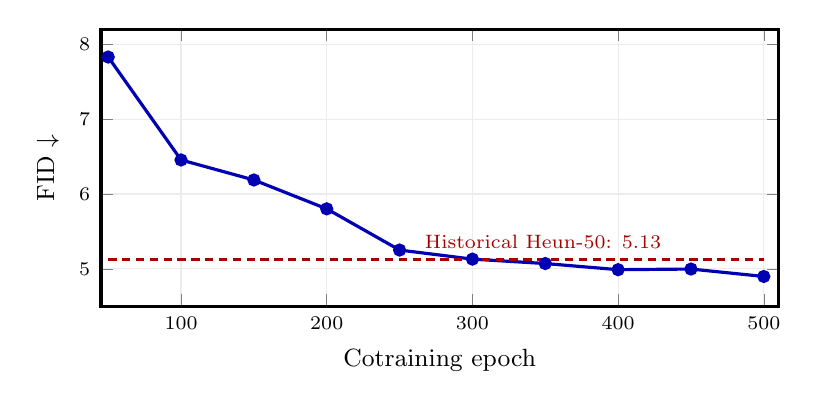
\begin{tikzpicture}
\begin{axis}[width=.84\linewidth,height=5.1cm,xlabel={Cotraining epoch},ylabel={FID $\downarrow$},xmin=45,xmax=510,ymin=4.5,ymax=8.2,grid=major,grid style={gray!15},tick label style={font=\scriptsize},label style={font=\small},line width=1.15pt]
\addplot[blue!70!black,mark=*,mark size=1.8pt] coordinates {(50,7.82922) (100,6.45466) (150,6.18698) (200,5.80162) (250,5.25108) (300,5.13003) (350,5.07100) (400,4.98903) (450,4.99760) (500,4.89833)};
\addplot[red!65!black,densely dashed] coordinates {(50,5.13) (500,5.13)};
\node[anchor=south west,font=\scriptsize,red!65!black] at (axis cs:260,5.13) {Historical Heun-50: 5.13};
\end{axis}
\end{tikzpicture}
\end{center}
The direct-latent run first passes FID 5 at epoch 400 (4.9890), gives 4.9976 at 450, and achieves its best reported FID \textbf{4.8983 at epoch 500}; posterior-reconstruction FID at the endpoint is 3.5726, while generating the child under an encoded root gives FID 3.9943. A historical flat terminal-KL run had FID 5.13 with Heun-SDE 50 steps; the exact provenance of an older approximately 5.04 claim was not recovered, and an approximately 4.97 oracle-start figure does not satisfy Gaussian initialization. The present result improves over both the directly documented 5.13 and the unverified approximately 5.04, \emph{subject to backend consistency and single-seed uncertainty}. It is an internal experimental record, not an external benchmark or a matched-parameter causal comparison. The new cascade uses two serial reverse solves, so 20 steps per head does not mean the same inference cost as 20 steps of a flat head.

\subsection{Learned allocation of stochastic representation}
The 64 root coordinates incur a growing fraction of the \emph{dimension-summed} terminal Gaussian-reference penalty, while the 192 child coordinates remain meaningfully used in reconstruction. Log-reported posterior variances, per-coordinate CSEM losses and the root's share of the terminal KL are:
\begin{center}
\begin{tabular}{@{}rrrrrr@{}}
\toprule
Epoch & $v_1$ & $v_2$ & $\ell_1$ & $\ell_2$ & Root share $K_T$ \\
\midrule
50 & 0.670 & 0.780 & 0.0295 & 0.0298 & 56.8\% \\
100 & 0.598 & 0.705 & 0.0310 & 0.0286 & 57.4\% \\
200 & 0.507 & 0.652 & 0.0323 & 0.0263 & 60.2\% \\
300 & 0.431 & 0.631 & 0.0338 & 0.0247 & 60.8\% \\
400 & 0.378 & 0.602 & 0.0343 & 0.0233 & 62.4\% \\
500 & 0.362 & 0.596 & 0.0346 & 0.0229 & 62.5\% \\
\bottomrule
\end{tabular}
\end{center}

The root posterior mean variance drops from 0.6704 to 0.3615 while the child falls from 0.7799 to 0.5961. The root's terminal KL per coordinate rises from 0.036997 to 0.039675, whereas the child's falls from 0.009396 to 0.007940. Accordingly its fraction of the dimension-summed $K_T$ budget increases from approximately 56.8\% to 62.5\%, although it contains only 25\% of the coordinates. The training-score loss for root rises (0.02952 to 0.03455) as the child loss falls (0.02975 to 0.02286); total per-coordinate score loss falls (0.02969 to 0.02578). These are \emph{mixed intrinsic CSEM information and score-head approximation} losses; a rising root loss does not establish deteriorating root score estimation, and terminal KL is \emph{not} mutual information $\II(X;Z_i\mid Z_{<i})$. The figures motivate a compact informative root plus conditionally modeled detail channel but do not prove a global/local semantic split.
\begin{center}
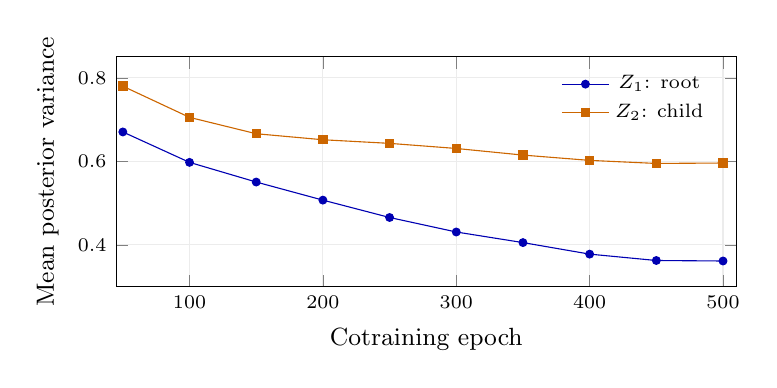
\begin{tikzpicture}
\begin{axis}[width=.78\linewidth,height=4.5cm,xlabel={Cotraining epoch},ylabel={Mean posterior variance},xmin=45,xmax=510,ymin=.30,ymax=.85,grid=major,grid style={gray!15},tick label style={font=\scriptsize},label style={font=\small},legend pos=north east,legend style={font=\scriptsize,draw=none,fill=none}]
\addplot[blue!70!black,mark=*,mark size=1.4pt] coordinates {(50,0.67040) (100,0.59759) (150,0.55053) (200,0.50722) (250,0.46566) (300,0.43095) (350,0.40558) (400,0.37799) (450,0.36271) (500,0.36153)};\addlegendentry{$Z_1$: root}
\addplot[orange!80!black,mark=square*,mark size=1.5pt] coordinates {(50,0.77993) (100,0.70533) (150,0.66613) (200,0.65172) (250,0.64309) (300,0.63086) (350,0.61503) (400,0.60235) (450,0.59500) (500,0.59605)};\addlegendentry{$Z_2$: child}
\end{axis}
\end{tikzpicture}
\end{center}
\subsection{Endpoint child interventions and generative fidelity}
At epoch 500, a fixed 128-image intervention holds the encoded root unchanged and varies only the child. Measurements are decoded-image MSE and perceptual distance to the original image:
\begin{center}
\begin{tabular}{@{}lrrr@{}}
\toprule
Child variant & MSE to input & MSE to posterior decode & LPIPS to input\\
\midrule
Posterior $Z_2$ & 0.01341 & 0 & 0.03691\\
Zero $Z_2$ & 0.05056 & 0.04408 & 0.10858\\
Shuffled posterior $Z_2$ & 0.07272 & 0.06672 & 0.13062\\
Generated conditional draw 1 & 0.06530 & 0.05839 & 0.10055\\
Generated conditional draw 2 & 0.06614 & 0.05965 & 0.10338\\
\bottomrule
\end{tabular}
\end{center}
Two independent generated children decoded at the same root differ by image MSE 0.04712 (posterior vs. generated draw 1: 0.05839). Zeroing the child raises input MSE by a factor 3.77; shuffling raises it by a factor 5.42. The child is therefore \emph{not} ignored, even as its conditional score loss decreases. An independently generated child need not reconstruct the particular $x$ used to select the encoded root; these paired changes measure intervention sensitivity and conditional diversity, not a calibrated conditional-distribution goodness-of-fit test.

\subsection{Gradient routes, cutoff and numerical sensitivity}
The epoch-500, 16-image, evaluation-mode gradient check (online score heads) confirms a child-CSEM gradient into \emph{both} posterior levels: the root/child posterior norms from the child score term are 0.00494/0.01312; the child head norm is 0.02314. The root's own CSEM term yields root-posterior norm 0.00615 and no child-posterior gradient. Pixel reconstruction gives root/child posterior norms 0.00768/0.01830, and the perceptual term gives 0.01452/0.03102. The measured full-VAE reconstruction--CSEM gradient cosine is $-0.104$, and the predicted joint clip factor is 1.0 on that batch. These values do not give optimizer-step sizes or global clipping frequency.

All logged fractions of posterior log variances below the small-time scale $\log\delta_0=-10.128$ (and the deeper cutoff) are zero for both blocks throughout 500 epochs. The automatic band penalty is therefore acting far from a sharp-collapse regime; its gradient is tiny in the endpoint probe. In a separately reported paired 1,024-image sampling check at epoch 500, CFG 3 / RK4-20 gives FID 24.584; CFG 1 / RK4-20 gives 25.796; CFG 3 / RK4-40 gives 24.444. The 1,024-image FIDs are \emph{not directly comparable} to the 10,000-image principal FID, but the matched checks suggest little gain from doubling solver steps relative to the effect of conditioning/guidance.

\newpage
\section{Evaluation, generation and next controlled tests}
\subsection{Sequential generation and evaluation discipline}
Sample $Z_1$ from its full-horizon reverse OU diffusion, hold the completed root fixed, then sample $Z_2\mid Z_1$ using a second conditional reverse diffusion, and decode the two generated codes directly (no post-score child baseline/scale map). The conditional head's spatial projections can be cached for each child reverse trajectory. Integration stops at the small positive $t_{\min}$, so the completed root used as ``clean'' conditioning has a negligible but nonzero endpoint discrepancy. Terminal KL anchors the finite-$T$ Gaussian initialization separately from the cutoff term.

Save and compare, with the same 10,000-image FID backend and sampling settings, the full generative FID, posterior reconstruction FID and encoded-root/generated-child FID. Keep 1,024-image solver/CFG checks as separate within-subset diagnostics; maintain fixed bank, labels, model EMA and sample count across alternatives. Include child-zero/shuffle/generated interventions and direct gradient-routing tests. Track time-resolved root/child CSEM losses and a separate estimate of head approximation error if aiming to measure conditional information rather than infer it from training loss.

\subsection{Open causal questions}
\begin{enumerate}
\item \textbf{Direct child versus residual affine predecessor.} Run from-scratch matched sweeps with identical schedules, head budgets, decoder capacities and noisy-root reconstruction. The present 4.898 versus 5.341 comparison changes more than one architectural choice and stops at different epochs; it is not an isolated transformation ablation.
\item \textbf{Flat versus cascade with capacity and latency control.} Compare the direct $64+192$ two-block model against the 256-coordinate flat VAE under common evaluation, with multiple seeds, matched parameter/FLOP budgets, and \emph{serial} total NFE or wall clock, not only 20 steps per reverse solve. An LSGM-style joint-latent prior on the same frozen hierarchy would isolate joint versus factorized score learning.
\item \textbf{Information allocation.} Measure the canonical per-block OU-time CSEM integral and, where feasible, an independently estimated aggregate score-head error to bound $\II(X;Z_1\mid C)$ and $\II(X;Z_2\mid Z_1,C)$. Terminal KL fractions and posterior variances are not those mutual informations. Use root/child swaps or conditional grids to establish whether $Z_1$ primarily encodes large-scale semantics and $Z_2$ local detail.
\item \textbf{Loss and schedule ablations.} With the direct-$Z_2$ architecture fixed, vary representation-specific versus head CSEM weights, $B_{t_{\min}}$, decoder corruption time, and conditional child network capacity, keeping the learning schedule explicit. A continuation from a finished cosine schedule needs a deliberate LR continuation policy, not merely a higher epoch count.
\end{enumerate}

\textbf{Updated conclusion.} The default Fashion-MNIST cascade is now the \emph{direct stochastic child} model. The full 500-epoch, 10,000-image Gaussian-start run finishes at \textbf{FID 4.8983}, our strongest documented terminal-KL CSEM result for FMNIST in this experimental record. The architecture preserves conditional Gaussian score targets, end-to-end root/child gradient coupling, and a reconstruction loss without clean-root bypass. It yields useful dependence on both latent blocks while remaining subject to standard single-seed and unmatched-compute limitations.


\vfill
{\footnotesize\textbf{Evidence record.} Updated from the supplied 500-epoch Fashion-MNIST direct-$Z_2$ stdout dated 13 October 2026 (500 training summaries, ten full 10,000-image evaluations, and 10 sets of child/solver/gradient diagnostics), current direct-latent training script, and earlier historical ablation records. Prior residual-innovation results are labeled historical. LSGM/NVAE motivate comparisons, but this implementation does not reproduce their full recipes.}
\end{document}
